%! Author = giaco
%! Date = 16/05/2024

\chapter{Method}
\label{sec:method}
The focus of this work is to simplify as much as possible the representation learning of current RL algorithms leveraging prior knowledge and letting the agent focus on learning the actual policy to solve the task.
Many previous works already, mentioned in Sec. \ref{sec:fm_rl}, share the idea of leveraging FMs to enhance the state representation facilitating the transfer of world knowledge and simplifying the RL training process.
Differently from these studies, our methodology is designed to use multiple models at the same time, instead of just one, to enhance the efficiency and effectiveness of RL agents by leveraging a set of pre-trained models tailored to the current task.

First, our work proposes a set of basic abilities like humans have.
RL agents are equipped with these FMs, which serve as the prior knowledge needed to generate diverse representations of the environment.
While agents interact with the environment, the current observation is collected and processed through each pre-trained model.
This process produces multiple perspectives or views of the world, each distinctively represented according to the particular model utilized.
These features embody various aspects of the environment, providing the agent with a comprehensive and enhanced understanding of the current state.

Then, we focus on how to effectively combine their latent representations to improve agents' performance.
The challenge lies in integrating these possible divergent views into a single and enriched representation.
In order to accomplish this, we employ a specialized combination module, that synthesizes the information from the various models into a single latent representation.
The intuition is that the enriched representation provides a comprehensive understanding of the current state of the environment, derived from the collective insights of the pre-trained models.
By utilizing FMs, our approach significantly alleviates the RL agent's need to learn the environmental representation from scratch, allowing it to focus more on refining the action-mapping process.
This not only accelerates the learning process but also enhances overall performance by providing a well-structured and informative representation.

The architecture of our agents is divided into two main components.
The first part takes care of processing the current observation into multiple latent representations and then combines them into a single enriched representation.
We refer to this part as the \textit{Feature Extractor} module.
The second part is the \textit{Policy Learning} network, where the unified representation is fed into a small fully-connected neural network whose responsibility is to map the latent encoding to actions.


In the following section, we will describe in detail how we designed the Feature Extractor module focusing on various combination techniques to merge the representations extracted by the FMs Sec.~\ref{sec:feature_extractor}.



% prova ad integrare se serve
%Besides our proposed methodology, we tested and compared the performance of several combination modules. All solutions act as interchangable modules inside the \texttt{Feature Extractor}, i.e. only need to replace the \textcolor{orange}{yellow} component in Figure \ref{fig:main_architecture}. Their output is a linear representation that is provided as input to the \texttt{Fully-Connected Network}. We report a rundown across all solutions:
%\begin{itemize}
%    \item \texttt{Linear} (LIN): pre-trained models' representations are linearized and concatenated.
%    \item \texttt{Fixed Linear} (FIX): embeddings are linearized to a predefined size, possibly using adapters to scale the information.
%    \item \texttt{Convolutional} (CNN): FMs' outputs are concatenated along the channel dimension. They are processed by a predefined number of convolutional layers and the resulting information is flattened to linear.
%    \item \texttt{Mixed} (MIX): this is a combination of the previous methods. Data coming from different spaces are dealt separately and then combined.
%    \item \texttt{Reservoir} (RES): inspired by \citet{gallicchio2017}, this approach leverages reservoir layers to combine models' representations.
%    \item \texttt{Dot Product Attention} (DPA): similarly to \texttt{Fixed Linear} the representations are reduced to a specific size - key and value. Via \texttt{scaled dot product attention} \citep{vaswani2017attention} we compute the final weighted representation using as query vector the representation obtained from the State Encoder.
%\end{itemize}








\section{Feature Extractor} \label{sec:feature_extractor}
The Feature Extractor module is the first part of our agent, it is responsible for processing the current observation and extracting a meaningful representation of the environment in a compact latent space.
It is composed of a set of pre-trained models, which are used to gather information from the environment and whose weights are frozen during the training process.
The second part of the module is the combination module, which is the core of the Feature Extractor.
We will talk about the implementation of the FMs in Sec. INSERT.

In this section instead, we will present one by one all the combination techniques that we have developed to merge the representations extracted by the FMs, with a particular emphasis on the Weight Sharing Attention module, which is the component that we propose as a solution to the problem of combining different FMs in an effective way, and we think that it deserves more relevance.


\subsection{Weight Sharing Attention}
\label{sec:wsa}

With a view to lifelong learning agents, the aim is therefore to equip the agent with prior skills that can be changed or improved over time to adapt to new unseen tasks.
To this end, a model capable of re-adapting to new abilities with little or no effort is needed.
To facilitate the integration of different pre-trained models, we propose WSA\@.
The WSA module leverages the concept of \textbf{weight sharing}, as seen for the first time in CNNs~\citep{fukushima1980neocognitron}, and \textbf{attention}~\citep{vaswani2017attention} principles to efficiently merge outputs from diverse FMs.
In specific, WSA dynamically adjusts the weights assigned to each pre-trained model based on the current context, emphasizing the most relevant models for the current state.

Supposing to have a set of $k$ pre-trained models $\Psi = \{\psi_1, \psi_2, \ldots, \psi_k\}$, each model $\psi_i$ is used to extract features from the current observation $\mathcal{O}$.
Each pre-trained model is equipped with an adapter $\mathcal{A}$, which is a small neural network consisting of a linear layer followed by a non-linearity layer, in this case, a ReLU activation function.
The adapter is used to learn a representation of the model's output and also to resize the latent representation of the FM to a fixed size, ensuring compatibility among different models.
As a result of this operation, each FM outputs an embedding $E_i$ of a predefined size.
The weights of the adapters are optimized during training.

Among the provided FMs, one model is used as \textbf{State Encoder} $\mathcal{E}$ to compute a representation of the current state, which serves as \textit{context} $\mathcal{C}$ for the attention mechanism.
Also for this model, the same kind of adapter is used to resize the latent representation to the same fixed size.


To compute the attention weights, we use a shared MLP $f_\theta$ that takes as input the context $\mathcal{C}$ concatenated with the single embedding $E_i$ of each FM\@.
This MLP outputs the model-specific weight $w_i$ to determine the contribution of each model in the final representation.
It is important to note that this MLP is shared across all models, ensuring uniform weight computation.
By dynamically adjusting weights based on the current context, WSA emphasizes the most relevant models for any given situation, resulting in a more accurate and adaptable representation.
The final representation $\mathcal{R}$ is computed using the weights for all pre-trained models and computing a weighted sum of their embeddings.
The output obtained is so a combination of the various perspectives, provided by the pre-trained models, into a single enriched latent representation.
This final representation is used for action mapping, enhancing the performance and learning efficiency of RL agents by integrating the strengths of multiple FMs.


Two additional features are guaranteed by the design approach.
WSA adds \textbf{explainability} to the model, where with explainability we mean the ability to understand the decision-making process of the agent.
In fact, by examining the weights assigned to different pre-trained models, we can gain insights into which models are most influential in a given context.
Additionally, WSA is \textbf{scalable} and \textbf{adaptable} to any number of pre-trained models.
Its shared component can handle any number of models, we can easily add or remove FMs from the set without the need to retrain the whole agent, making it a flexible solution for dynamically evolving agents.

Figure~\ref{fig:main_architecture} shows the main architecture of our agent, with an emphasis on the WSA module.
Algorithm~\ref{alg:wsa} instead reports the pseudocode for the actual implementation.

\begin{algorithm}[ht]
    \caption{Weight Sharing Attention}\label{alg:wsa}
    \texttt{In \textcolor{blue}{blue} we highlight the components that are updated during training.}\\
    \begin{algorithmic}[1]
        \Require Current observation $\mathcal{O}$, List of FMs $\Psi$, State Encoder $\mathcal{E}$
        \State $\mathcal{C} = \textcolor{blue}{\mathcal{A}_0}(\mathcal{E}(\mathcal{O}))$ \Comment{Compute current context representation}
        \For {FM $\psi$ in $\Psi$}
            \State $x = \psi_i(\mathcal{O})$ \Comment{Forward pass using current state}
            \State $E_i = \textcolor{blue}{\mathcal{A}_i}(x)$ \Comment{Use the adapters to compute the resized embedding}
            \State $w_i = \textcolor{blue}{f_\theta}(\mathcal{C}, E_i)$ \Comment{Compute the weight for current model using shared component}
        \EndFor
        \State $\mathcal{R} = \sum_{i=0}^{|\Psi|} w_i * E_i$ \Comment{Final representation: weights $W$, embeddings $E$ $\rightarrow$ $W \cdot E$}
    \end{algorithmic}
\end{algorithm}



\begin{figure}[ht]
    \begin{center}
        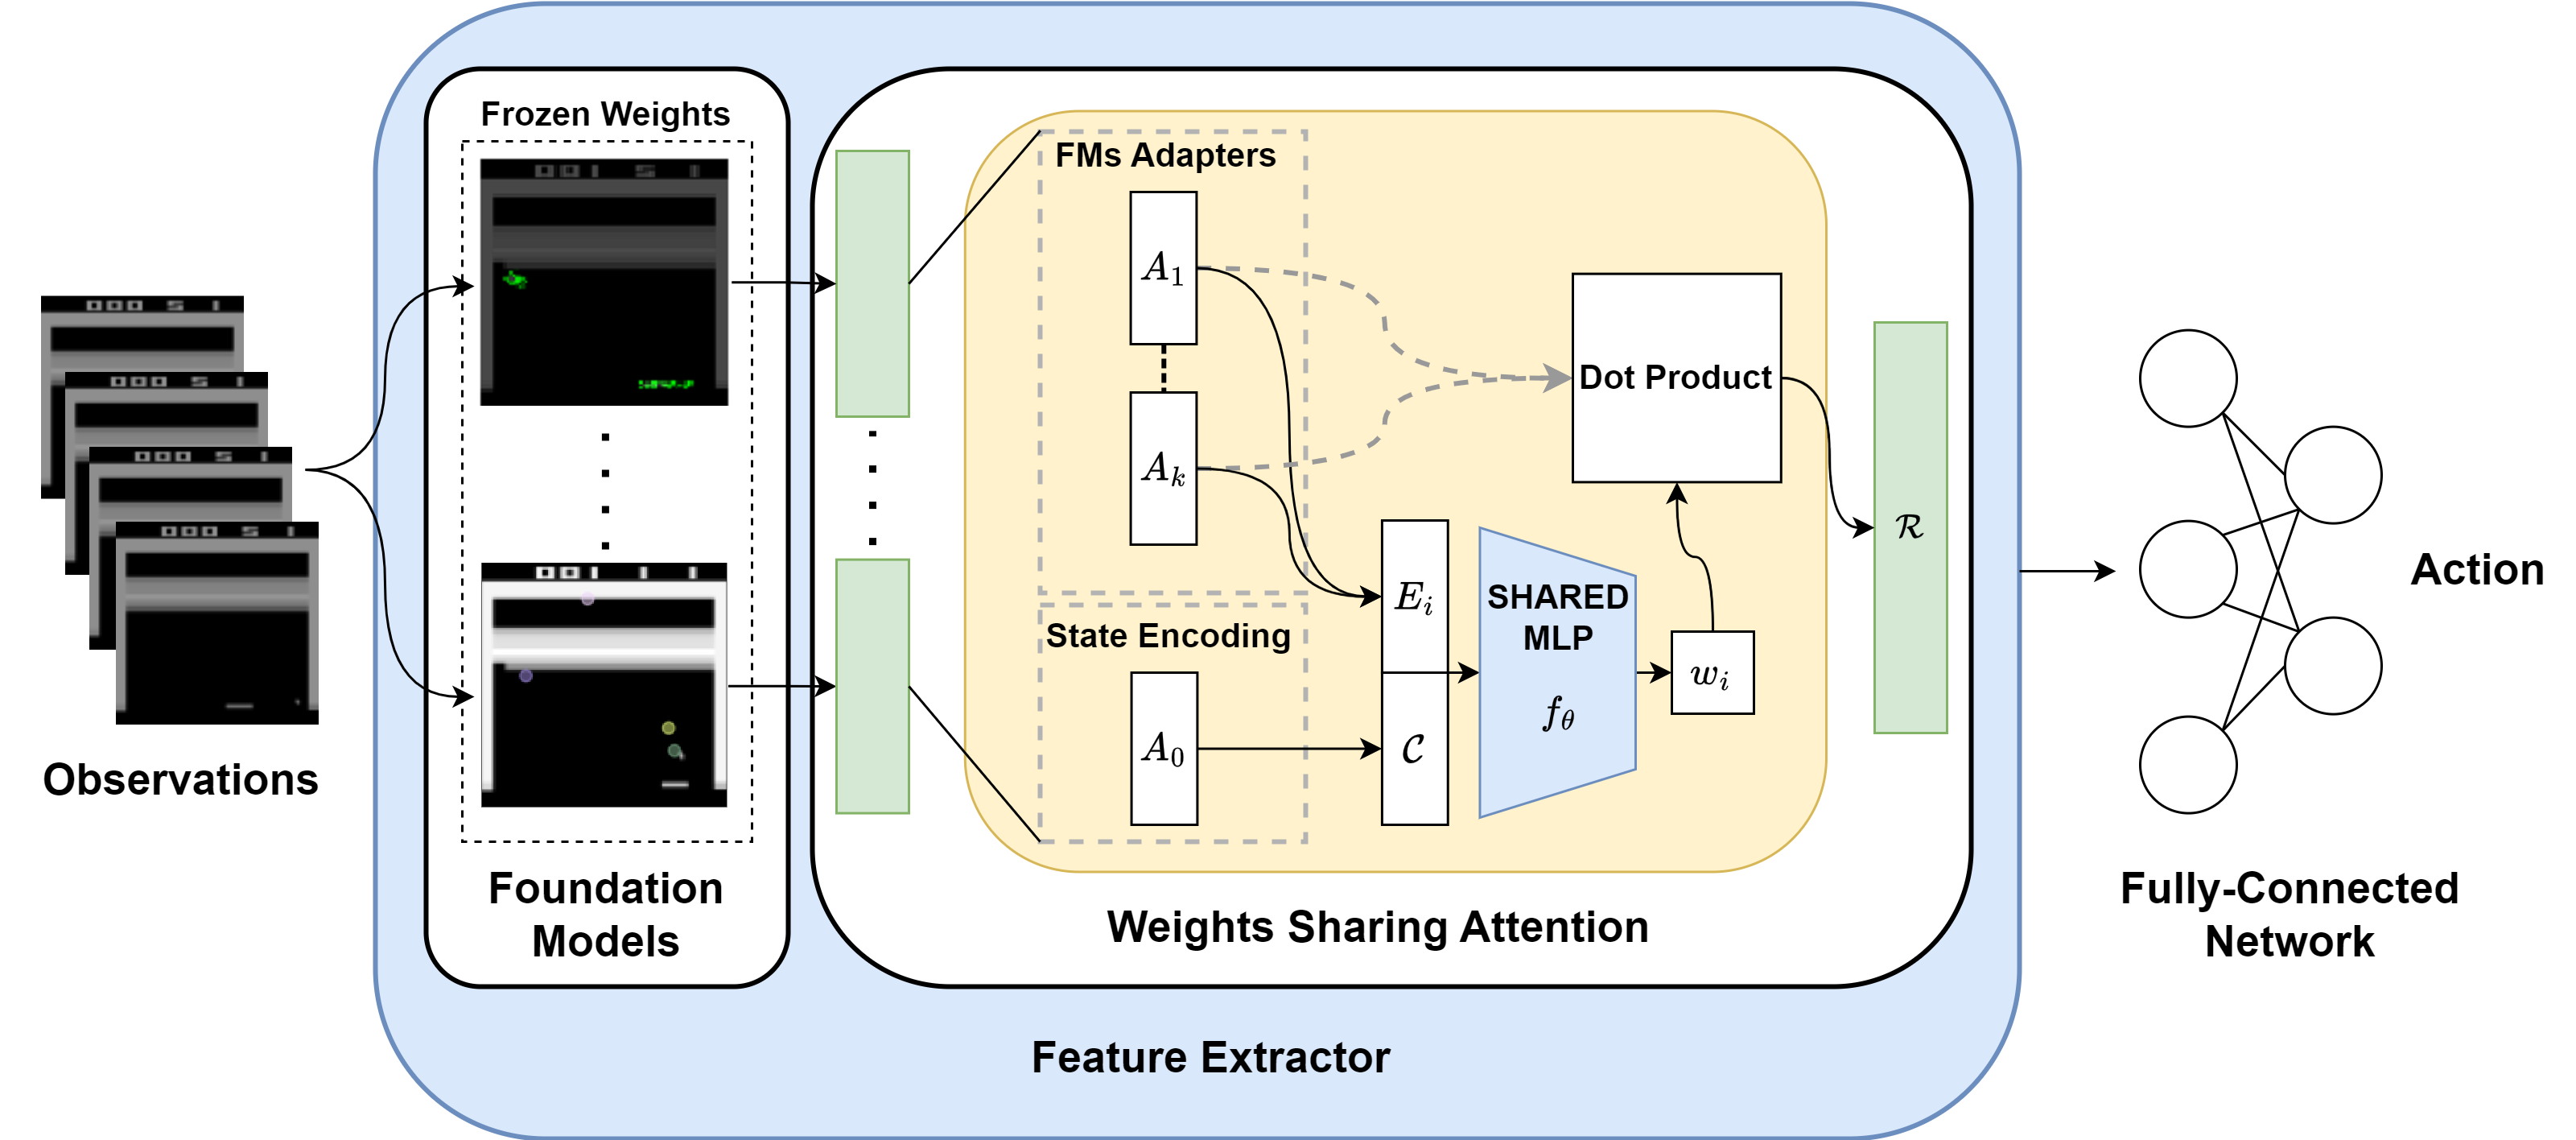
\includegraphics[width=1\textwidth]{images/main_architecture2}
    \end{center}
    \caption{In Figure we show all the information flow from observation to actions and the architecture of the WSA module. The last four frames are stacked together and passed as input to the FMs and their adapters $\mathcal{A}_1, \dots \mathcal{A}_k$ to obtain an embedding of the current state $E_i$. A State Encoder $\mathcal{E}$ and its adapter $\mathcal{A}_0$ compute an encoding of the state, that will be used as context $\mathcal{C}$. A shared MLP layer takes as input the context $\mathcal{C}$ and the representation of the $i^{th}$ FM, $E_i$, and produce the weight for that specific model. The final enriched representation $\mathcal{R}$ is obtained from the weighted summation between each weight $w_i$ and its respective embedding $E_i$. $\mathcal{R}$ is given as input to agents' \textit{Fully-Connected Network}.}
    \label{fig:main_architecture}
\end{figure}

\subsection{Linear Combination Modules}
\label{subsec:linear_combination}
Linear combination modules are the simplest way to merge the representations extracted by the FMs.
Considering the set of $k$ pre-trained models, each of them can output an embedding in the spatial field or a one-dimensional vector.
If the model outputs a one-dimensional vector, it is left as it is, while if it outputs a set of feature maps, it is flattened to produce a one-dimensional vector.
Then, the embeddings of each model are concatenated to create a large feature vector.
We refer to this module as \textit{LIN} for short.


One problem with this combination module is that the FMs may have very different dimensionality.
An embedding might be very large compared to the others, leading to a situation where one model becomes more important than the others just because its dimension is larger.
So, we developed another combination module, which we refer to as \textit{FIX}, where first we obtain a linear representation as in the previous module for each model.
Then, we map the representation of each model into an embedding of fixed dimensions using $k$ different linear layers with the same size.
Each linear layer is followed by a ReLU activation function.
The new embeddings are then concatenated as before and used as input for the rest of the network.

In Fig.~\ref{fig:lin_combination} we show the architecture of the two linear combination modules.


\begin{figure}[ht]
    \centering
    \begin{subfigure}[b]{0.47\textwidth}
        \centering
        \fbox{\rule[-.5cm]{0cm}{4cm} \rule[-.5cm]{4cm}{0cm}}
        %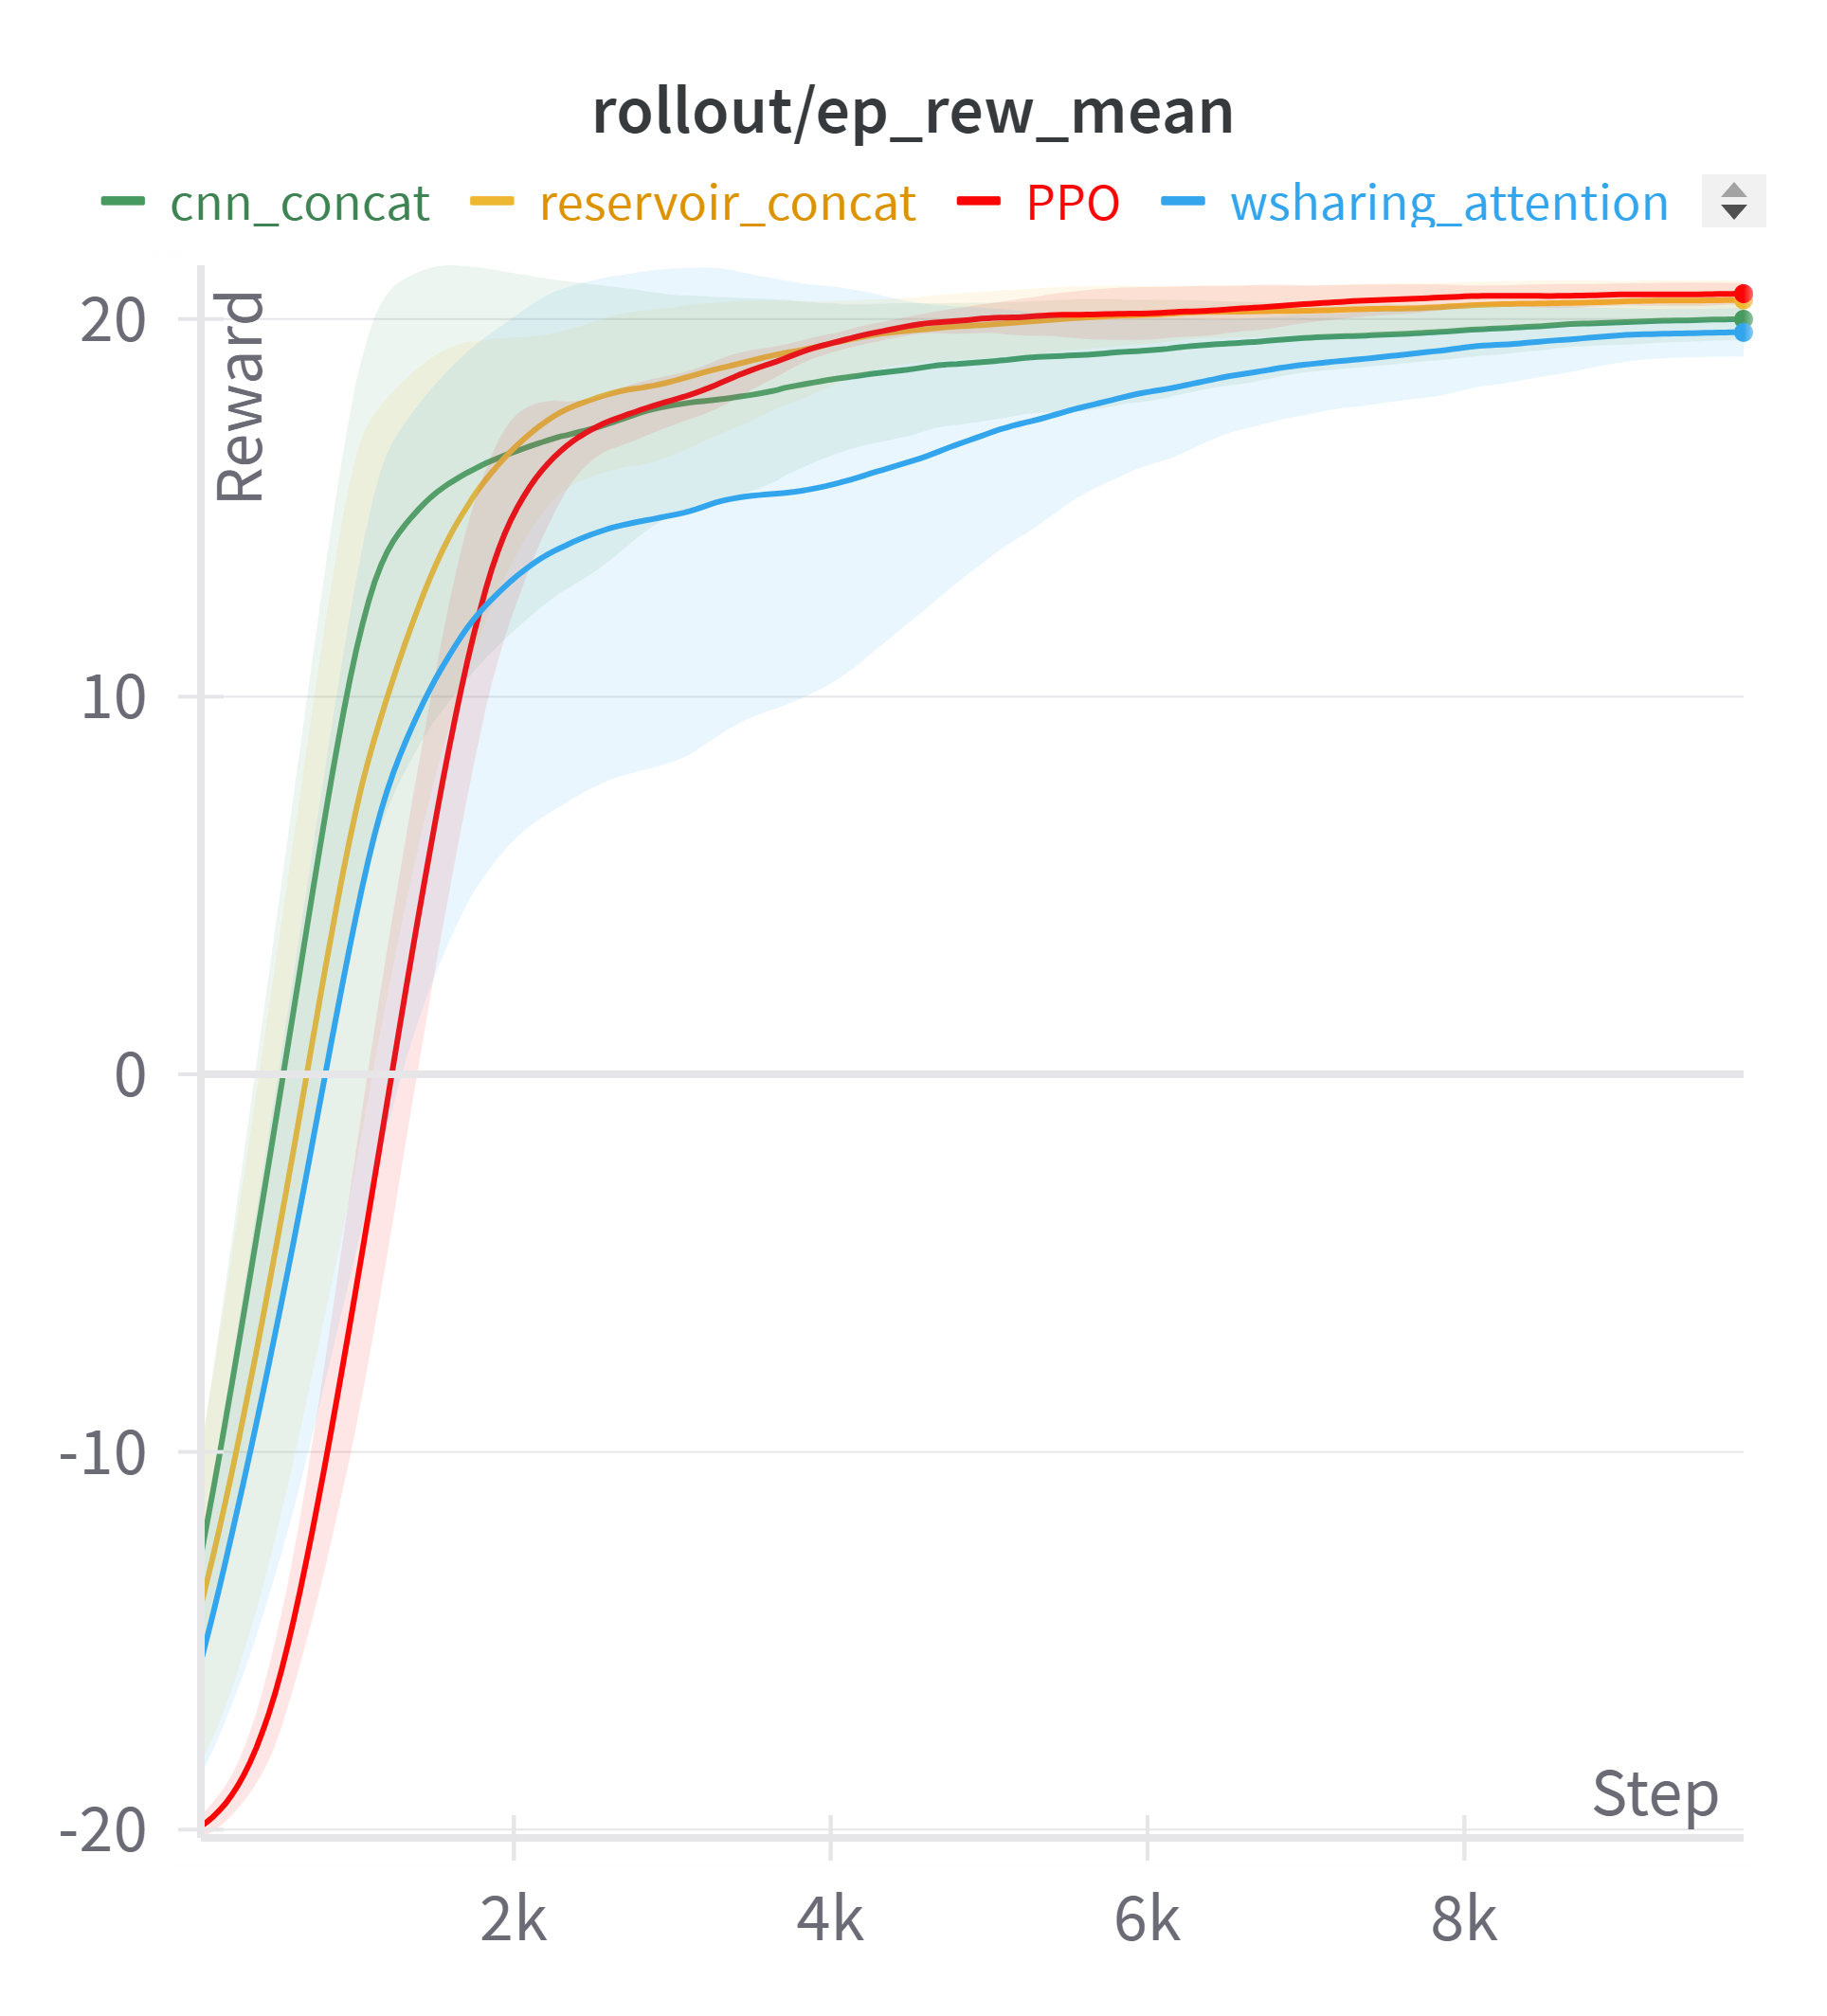
\includegraphics[width=\textwidth]{images/pong_train.png}
        \caption{\texttt{LIN}}
        \label{fig:lin}
    \end{subfigure}
    \hfill
    \begin{subfigure}[b]{0.47\textwidth}
        \centering
        \fbox{\rule[-.5cm]{0cm}{4cm} \rule[-.5cm]{4cm}{0cm}}
        %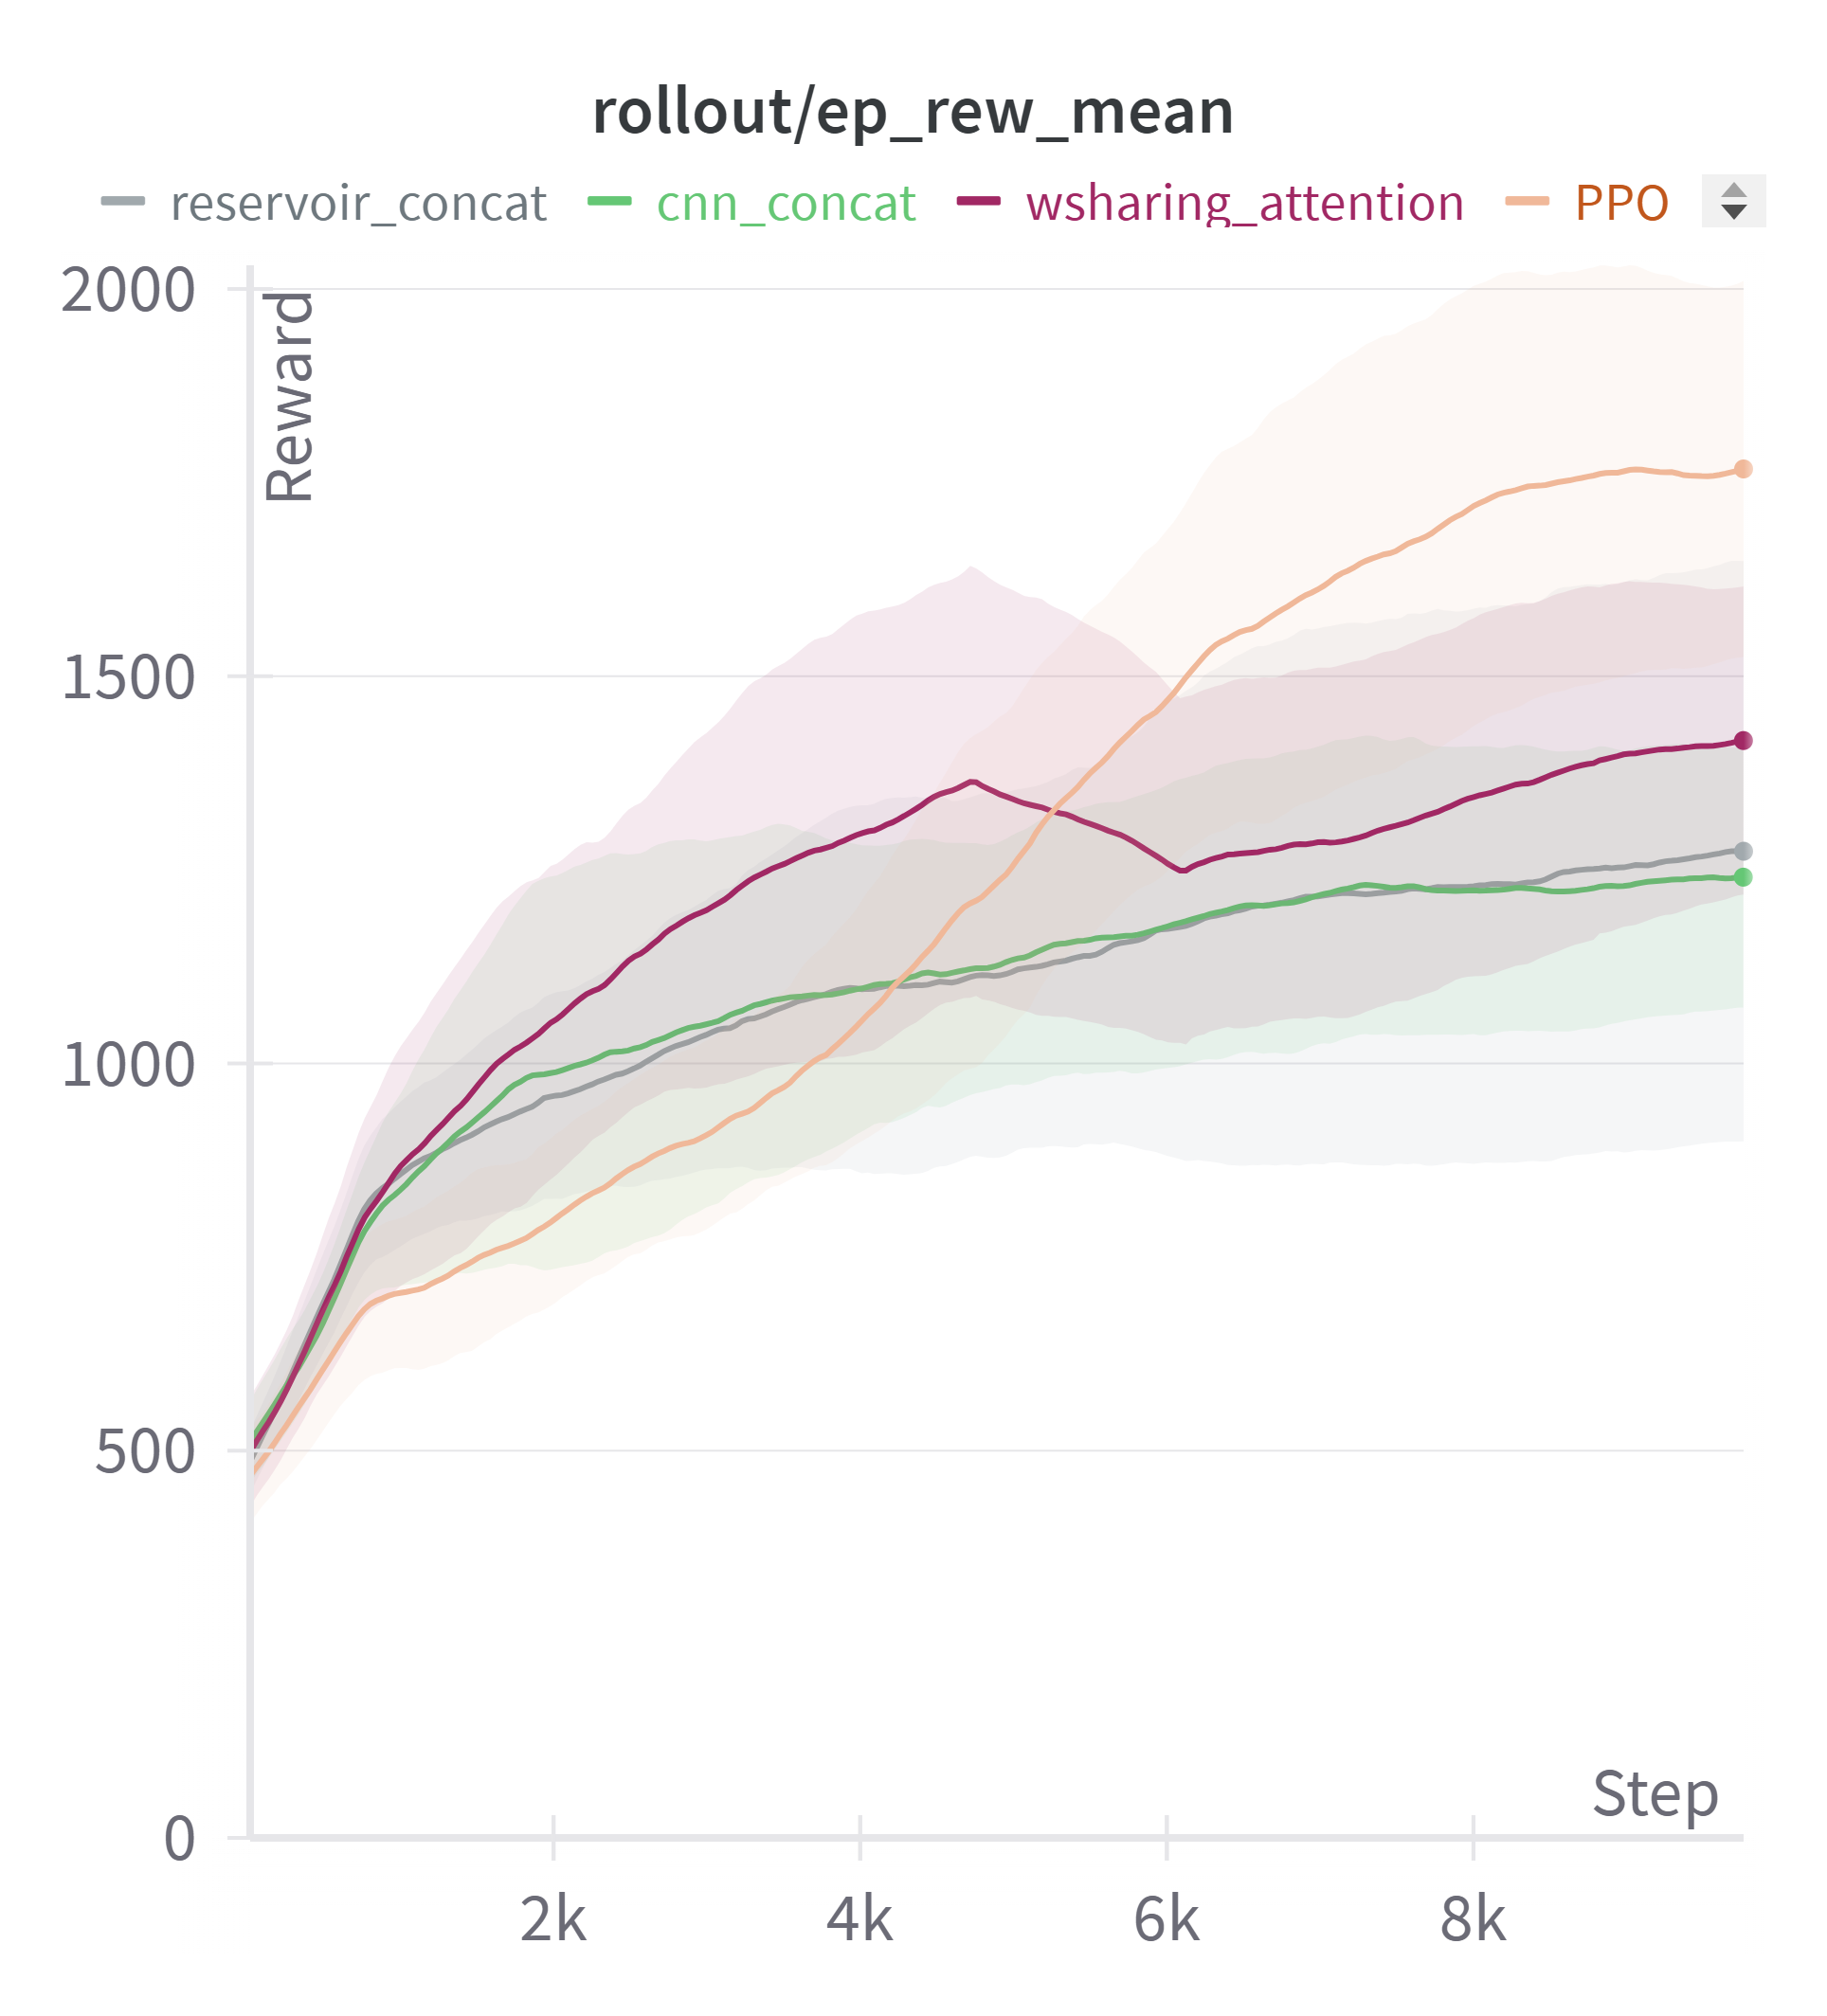
\includegraphics[width=\textwidth]{images/mspacman_train.png}
        \caption{\texttt{FIX}}
        \label{fig:fix_lin}
    \end{subfigure}

    \caption{In Figure we show the architecture of the Linear Combination Module (LIN) and the Fixed Linear Combination Module (FIX). In LIN, the embeddings of each model are concatenated to create a large feature vector. In FIX, the embeddings are mapped into an embedding of fixed dimensions using $k$ different linear layers with the same size.}
    \label{fig:lin_combination}
\end{figure}




\subsection{Convolutional Combination Modules}
\label{subsec:convolutional_combination}
In this combination module, we exploit the fact that FMs operate in the spatial field.
In fact, flatting the feature maps and concatenating them as in the linear combination modules may not be the best choice, as the spatial information is lost.
To overcome this issue, we first reshape the feature maps coming from the FMs to have the same dimensions.
FMs that output a one-dimensional vector are reshaped to match the dimensions of the other models.
Then, the reshaped embeddings are concatenated along the channel dimension and passed to one or more convolutional layers to extract features.
At this point, the output of the convolutional layer is flattened, and the embedding is passed to the rest of the network.
We refer to this combination module as \textit{CNN}.


Assuming that the set of FMs is composed of models that operate in the spatial field and models that operate in the linear one, we can exploit these two types of models to create a more complex combination module.
First, we concatenate the FMs that operate in the spatial field along the channel dimension and pass them through a convolutional layer, as for the previous module.
Then, we flatten the output of the convolutional layer and concatenate it with the embeddings of the linear models to create the final representation.
We call this combination module \textit{MIX} as it is a mixture of the previous two modules.

Figure~\ref{fig:conv_combination} shows the architecture of the two convolutional combination modules.

\begin{figure}[ht]
    \centering
    \begin{subfigure}[b]{0.47\textwidth}
        \centering
        \fbox{\rule[-.5cm]{0cm}{4cm} \rule[-.5cm]{4cm}{0cm}}
        %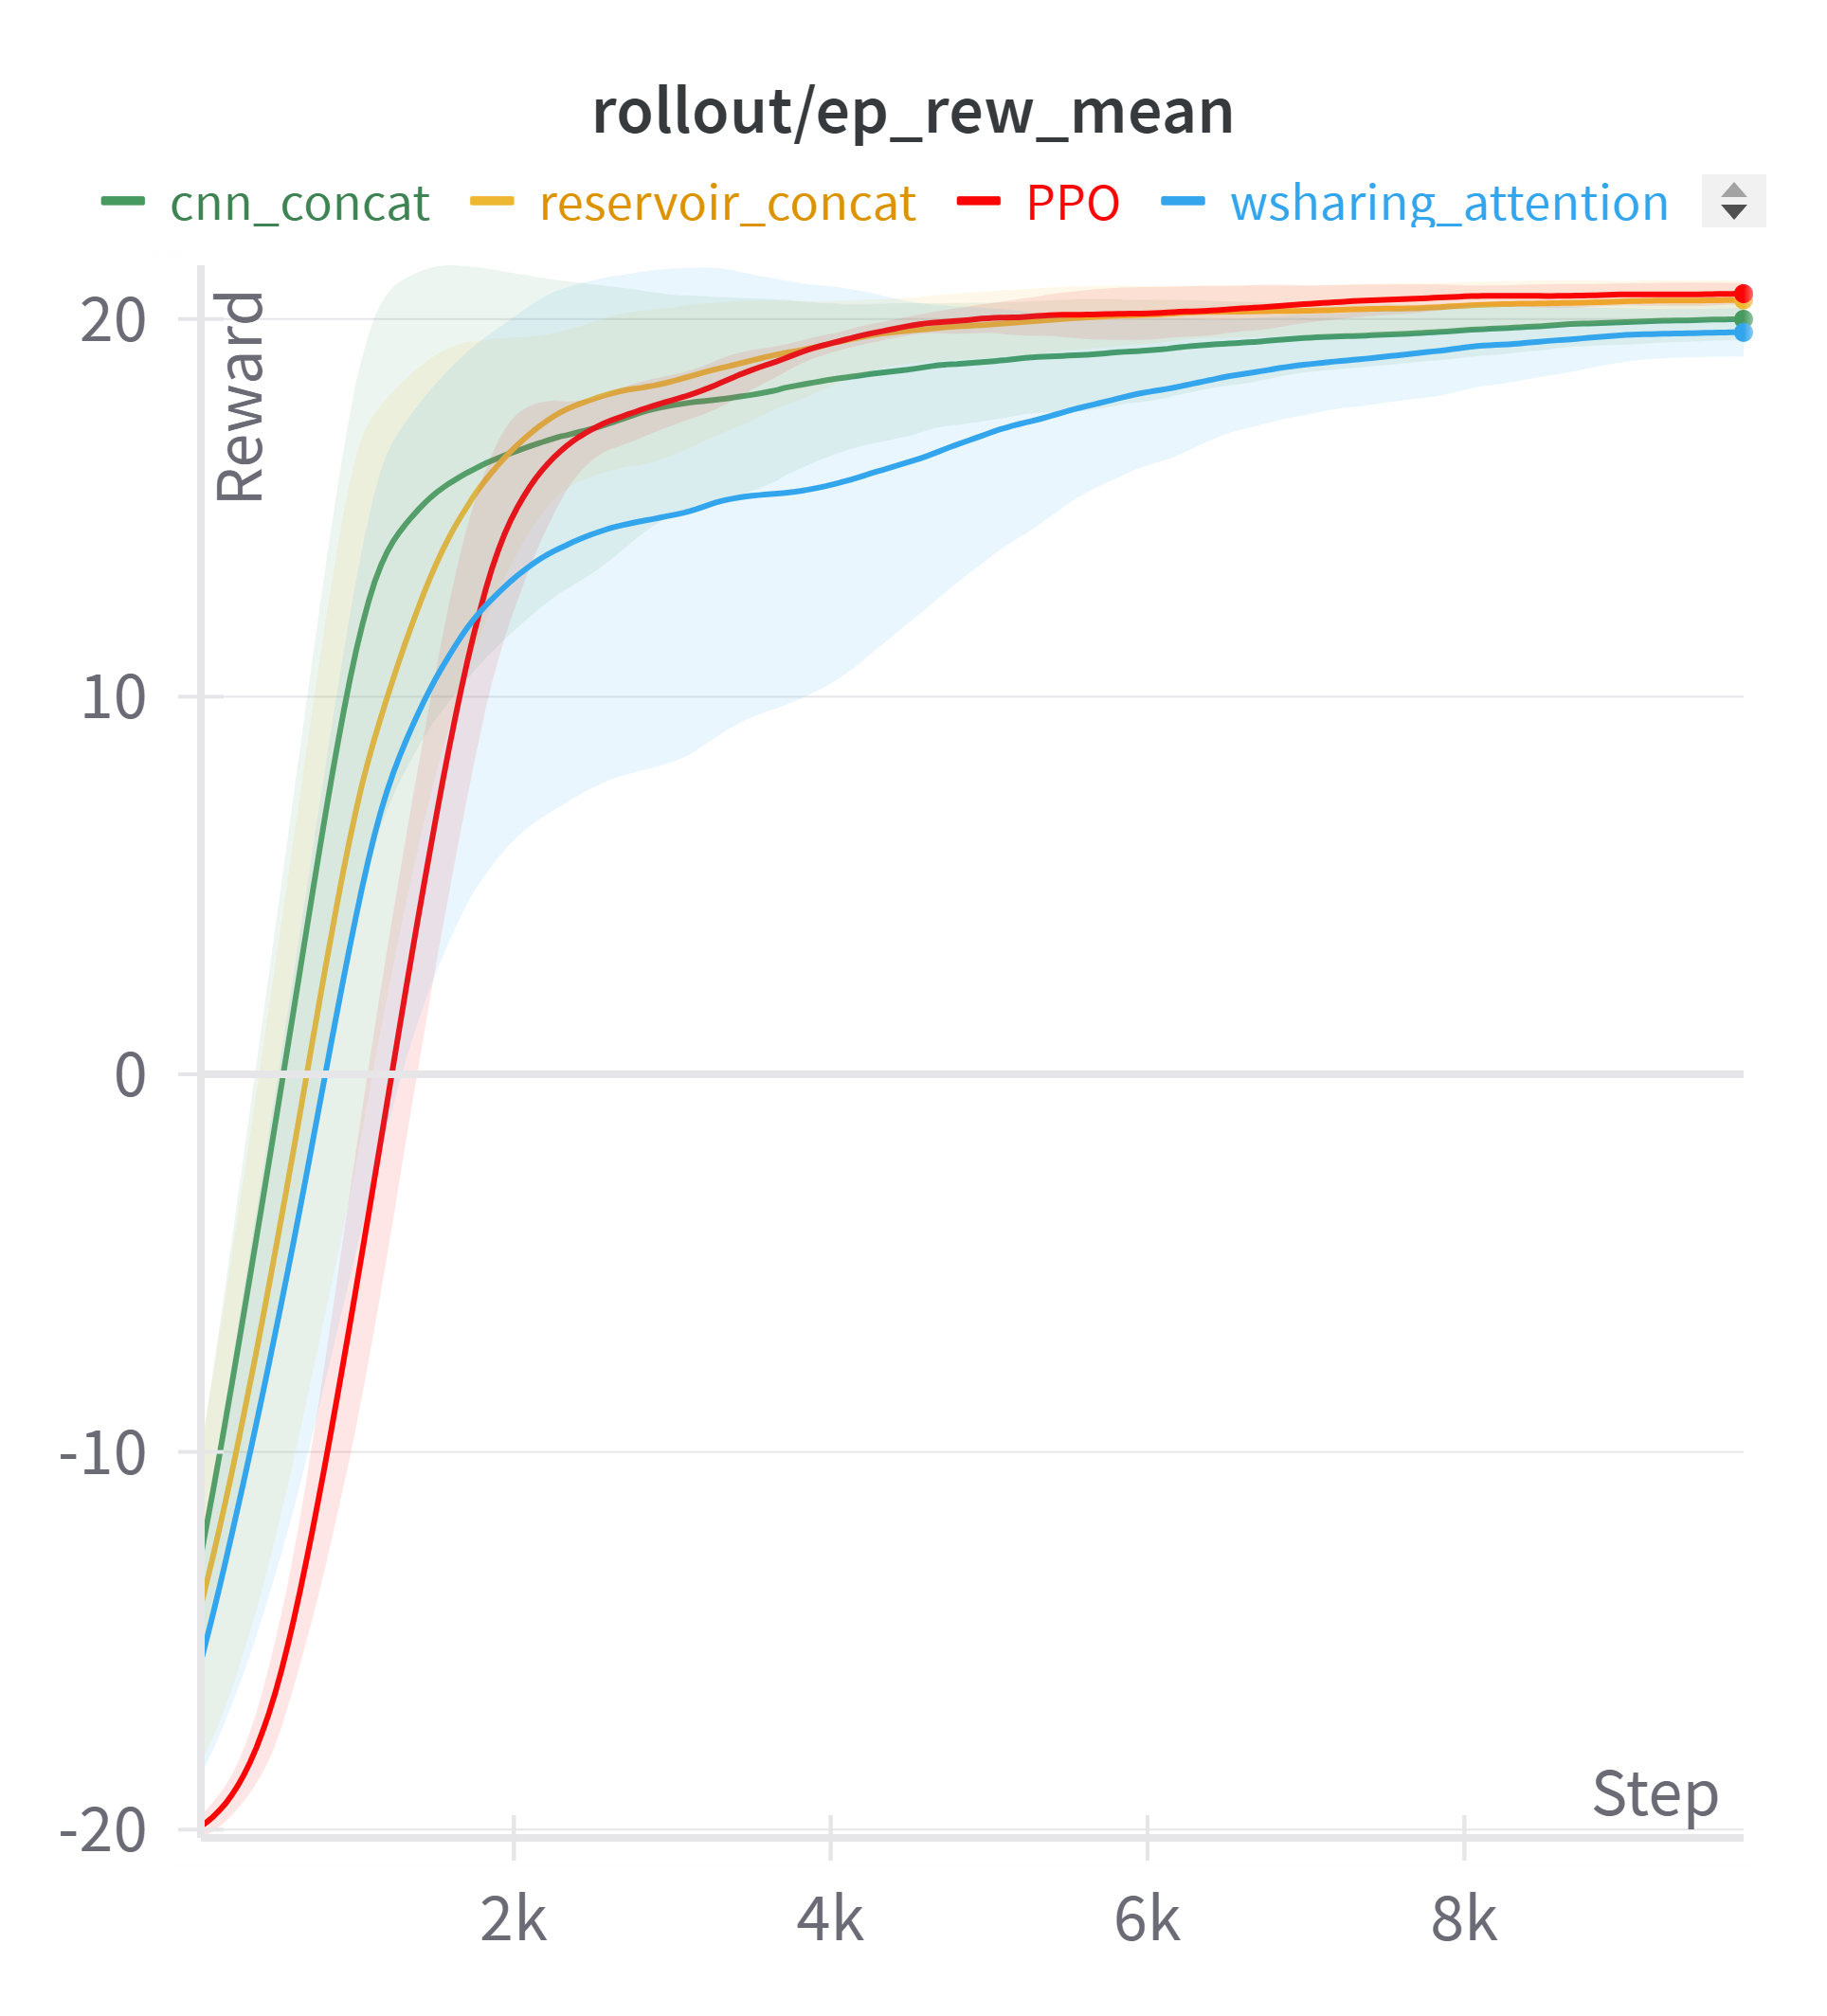
\includegraphics[width=\textwidth]{images/pong_train.png}
        \caption{\texttt{CNN}}
        \label{fig:cnn}
    \end{subfigure}
    \hfill
    \begin{subfigure}[b]{0.47\textwidth}
        \centering
        \fbox{\rule[-.5cm]{0cm}{4cm} \rule[-.5cm]{4cm}{0cm}}
        %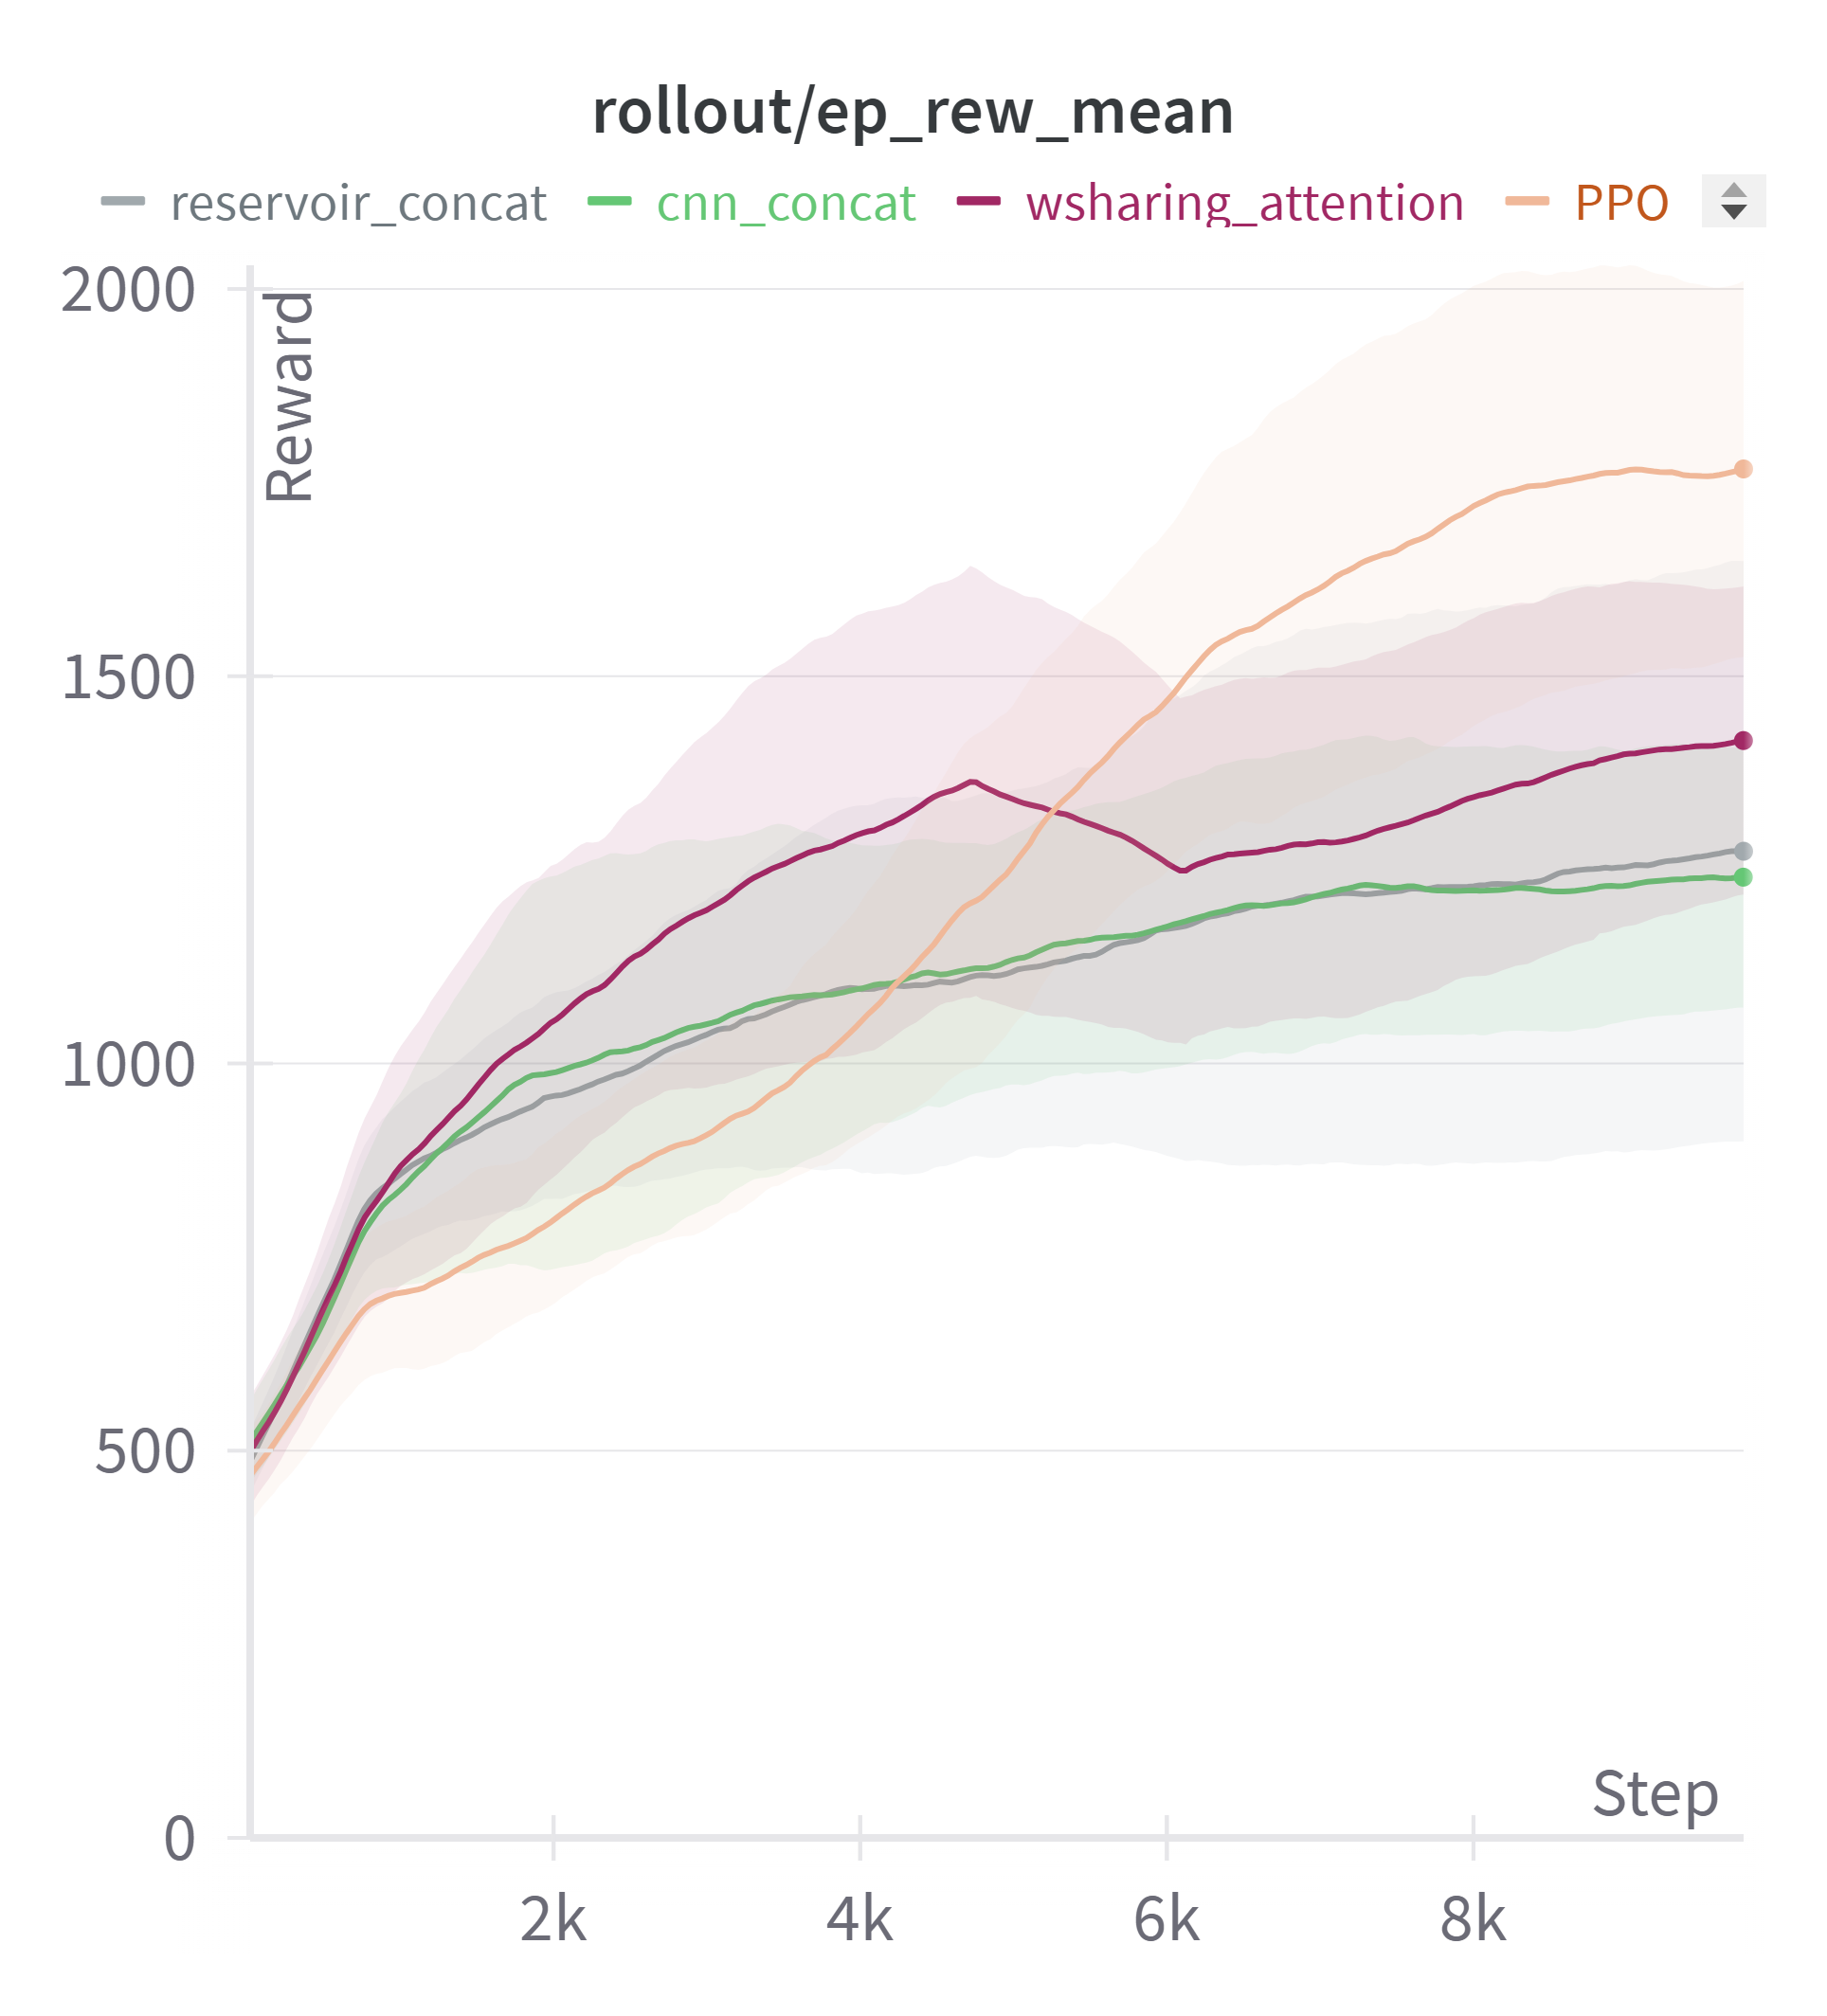
\includegraphics[width=\textwidth]{images/mspacman_train.png}
        \caption{\texttt{MIX}}
        \label{fig:mix}
    \end{subfigure}

    \caption{n Figure we show the architecture of the Convolutional Combination Module (CNN) and the Mixed Combination Module (MIX). In CNN, we concatenate the embeddings along the channel dimension. In MIX, we concatenate the spatial embeddings together and then we concatenate all the linear embeddings.}
    \label{fig:conv_combination}
\end{figure}

\subsection{Reservoir Combination Module}
\label{subsec:reservoir_combination}
Inspired by the work of \citet{gallicchio2017}, we decided to explore reservoir dynamics properties to map the input into a lower-dimension latent space using a non-linear transformation.
To develop this combination module, we created a reservoir with a fixed number of neurons, and as input, we used large embedding by concatenating the representations of the FMs as in LIN\@.
The output of the reservoir is a vector of the size of the reservoir, which is used as input to the policy learning network.
We refer to this combination module as \textit{RES}.
Figure~\ref{fig:reservoir_combination} shows the architecture of the reservoir combination module.

\subsection{DotProduct Attention Combination Module}
\label{subsec:dpa}

We also explored the possibility of combining representations using different types of attention-like mechanisms conditioned on the configuration of the environment.
In this case, we used the \textit{scaled dot product attention}~\citep{vaswani2017attention}.
As for the WSA module, the pre-trained model representations are reduced to a vector of fixed size.
These are then stacked together to form a tensor of shape $(k \times \text{vector\_size})$, where $k$ are the number of available FMs, and $vector\_size$ is the fixed dimension of each pre-trained model embedding.
This constitutes the \textbf{key} part and the \textbf{value} part of the attention module.
For the \textbf{query} part, as for the WSA module, we used the State Encoder to encode the current state of the game in a latent space, and we used an adapter to obtain a vector of the same dimensions.
This therefore represents the context.
As the name of the module suggests, the attention module first computes the dot product of the query with the keys, divided by the square root of the dimension of the query, then it uses a softmax function to obtain the weights.
Finally, the output of the module is computed as the dot product of the weights with the values.
We call this combination module \textit{DPA} and in Fig.~\ref{fig:dpa_combination} we show the architecture of the module.


\begin{figure}[ht]
    \centering
    \begin{subfigure}[b]{0.47\textwidth}
        \centering
        \fbox{\rule[-.5cm]{0cm}{4cm} \rule[-.5cm]{4cm}{0cm}}
        %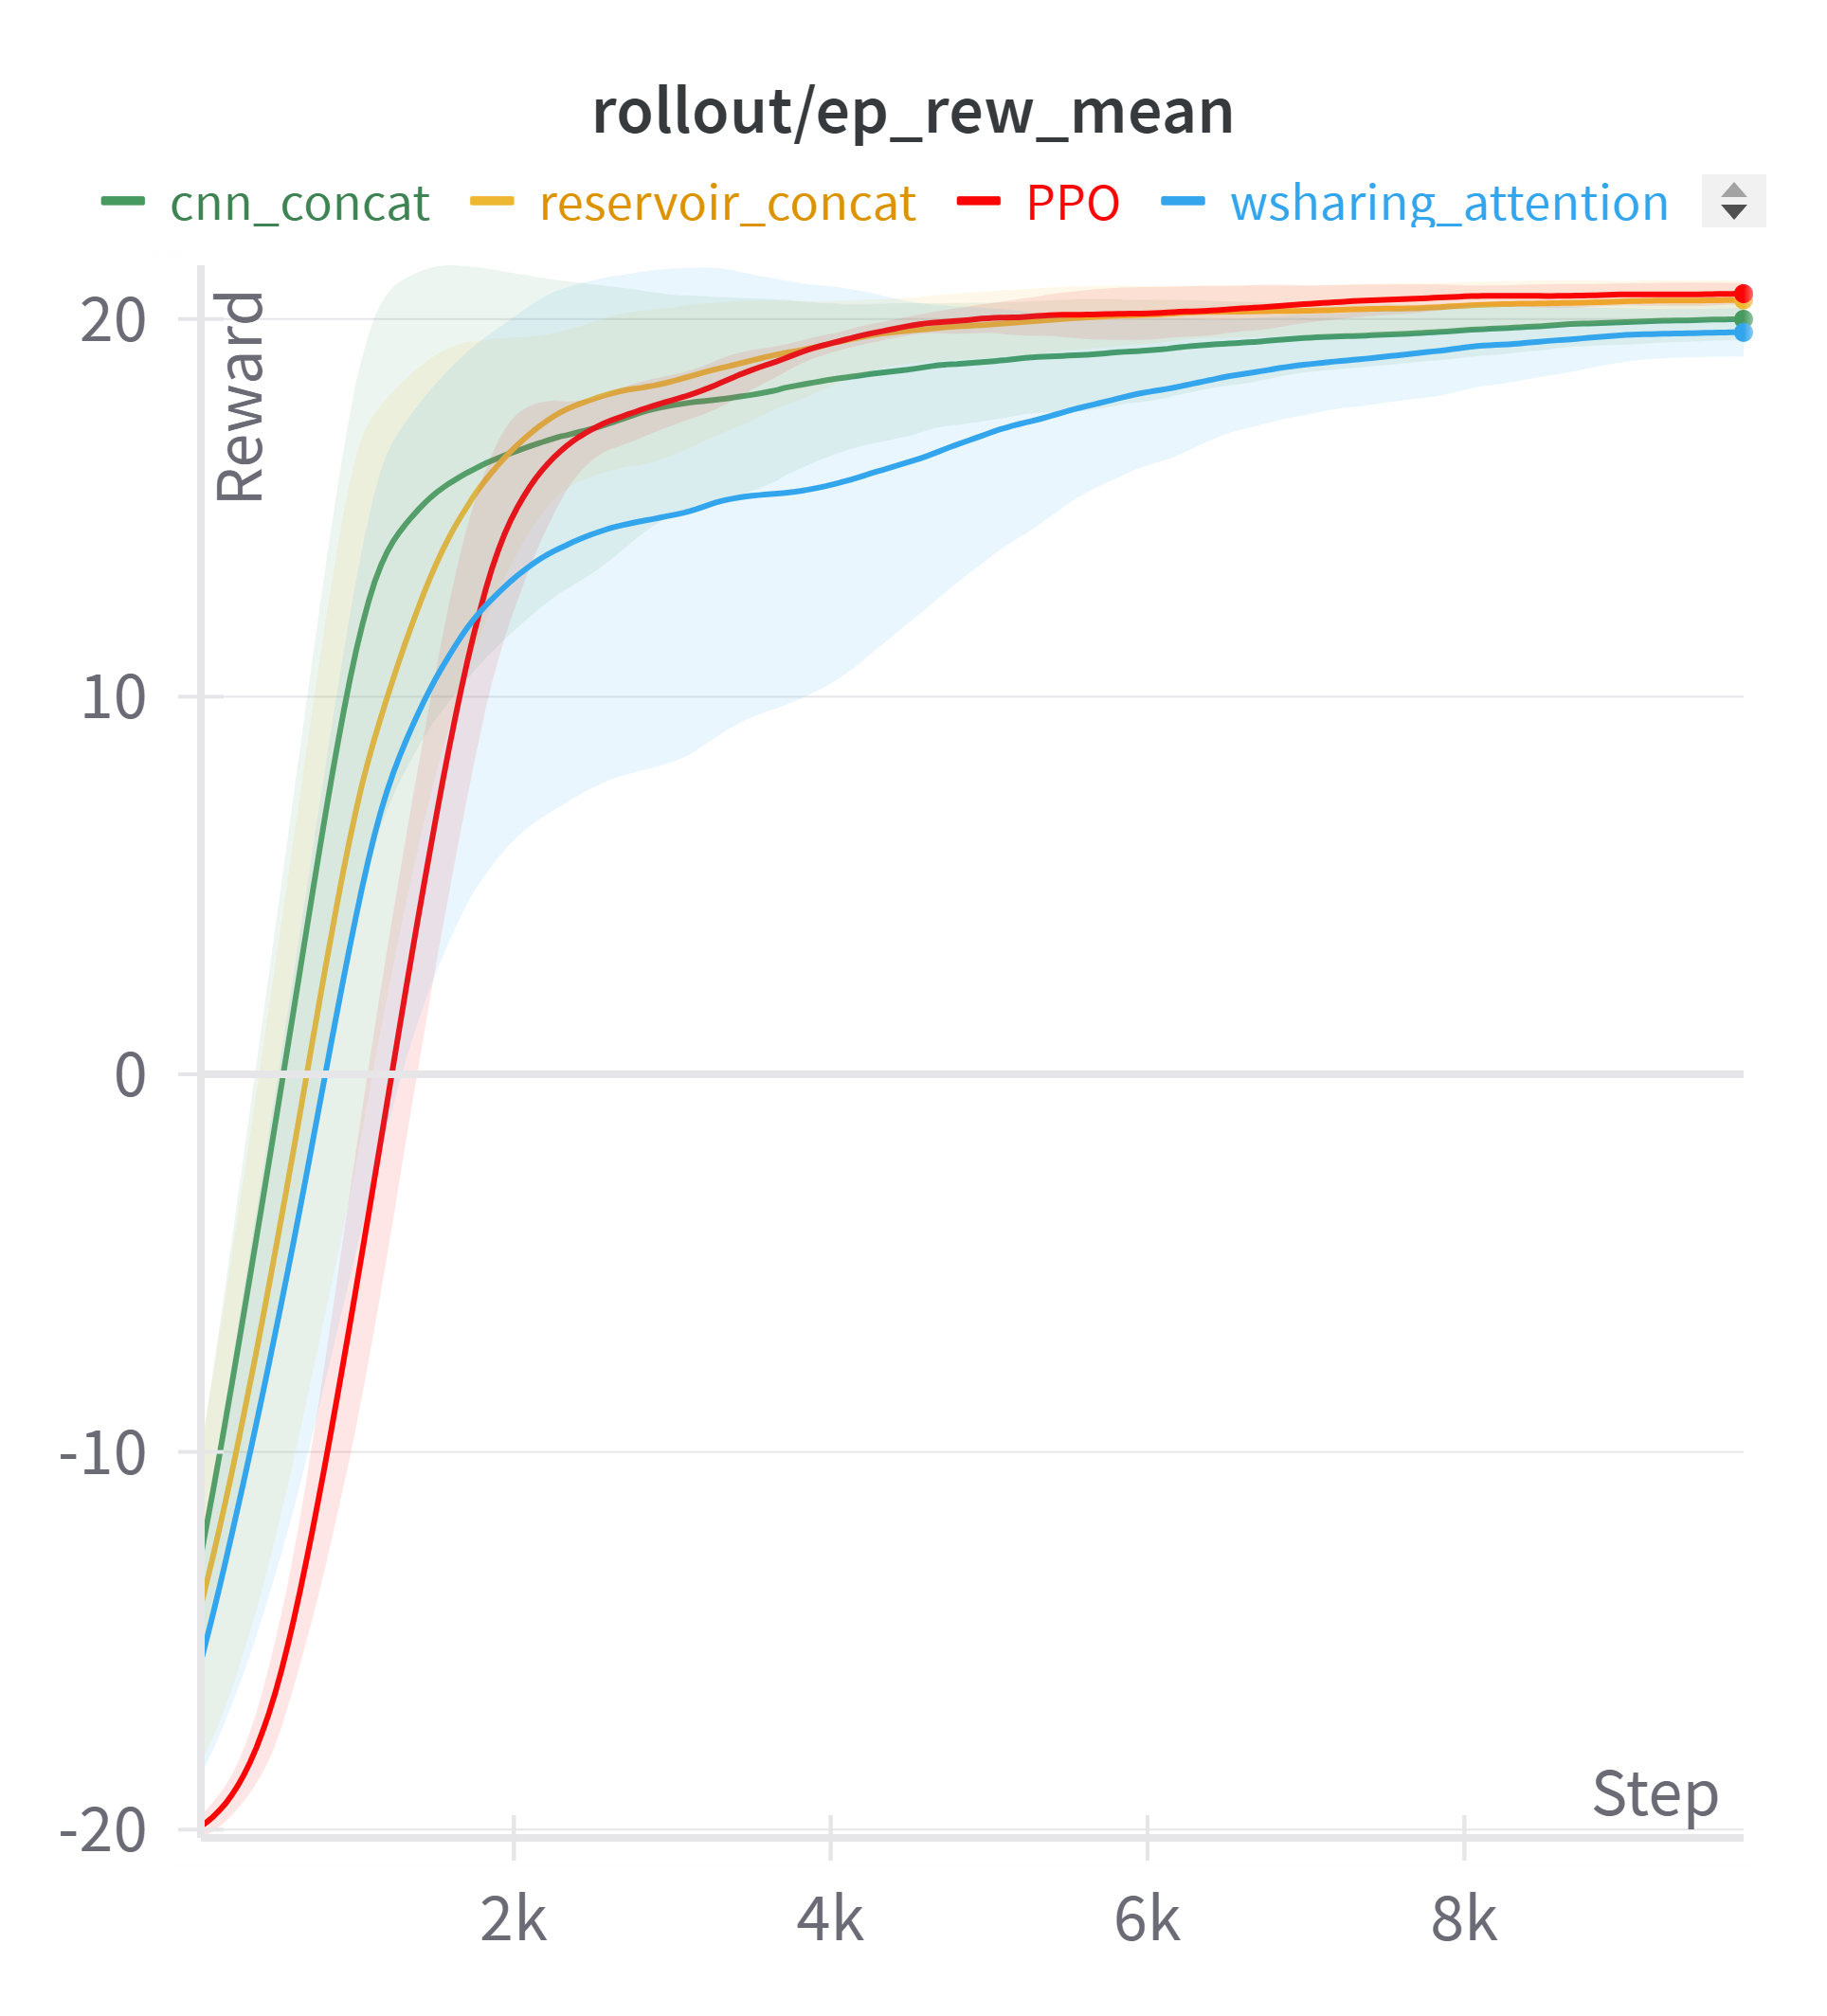
\includegraphics[width=\textwidth]{images/pong_train.png}
        \caption{\texttt{RES}}
        \label{fig:reservoir_combination}
    \end{subfigure}
    \hfill
    \begin{subfigure}[b]{0.47\textwidth}
        \centering
        \fbox{\rule[-.5cm]{0cm}{4cm} \rule[-.5cm]{4cm}{0cm}}
        %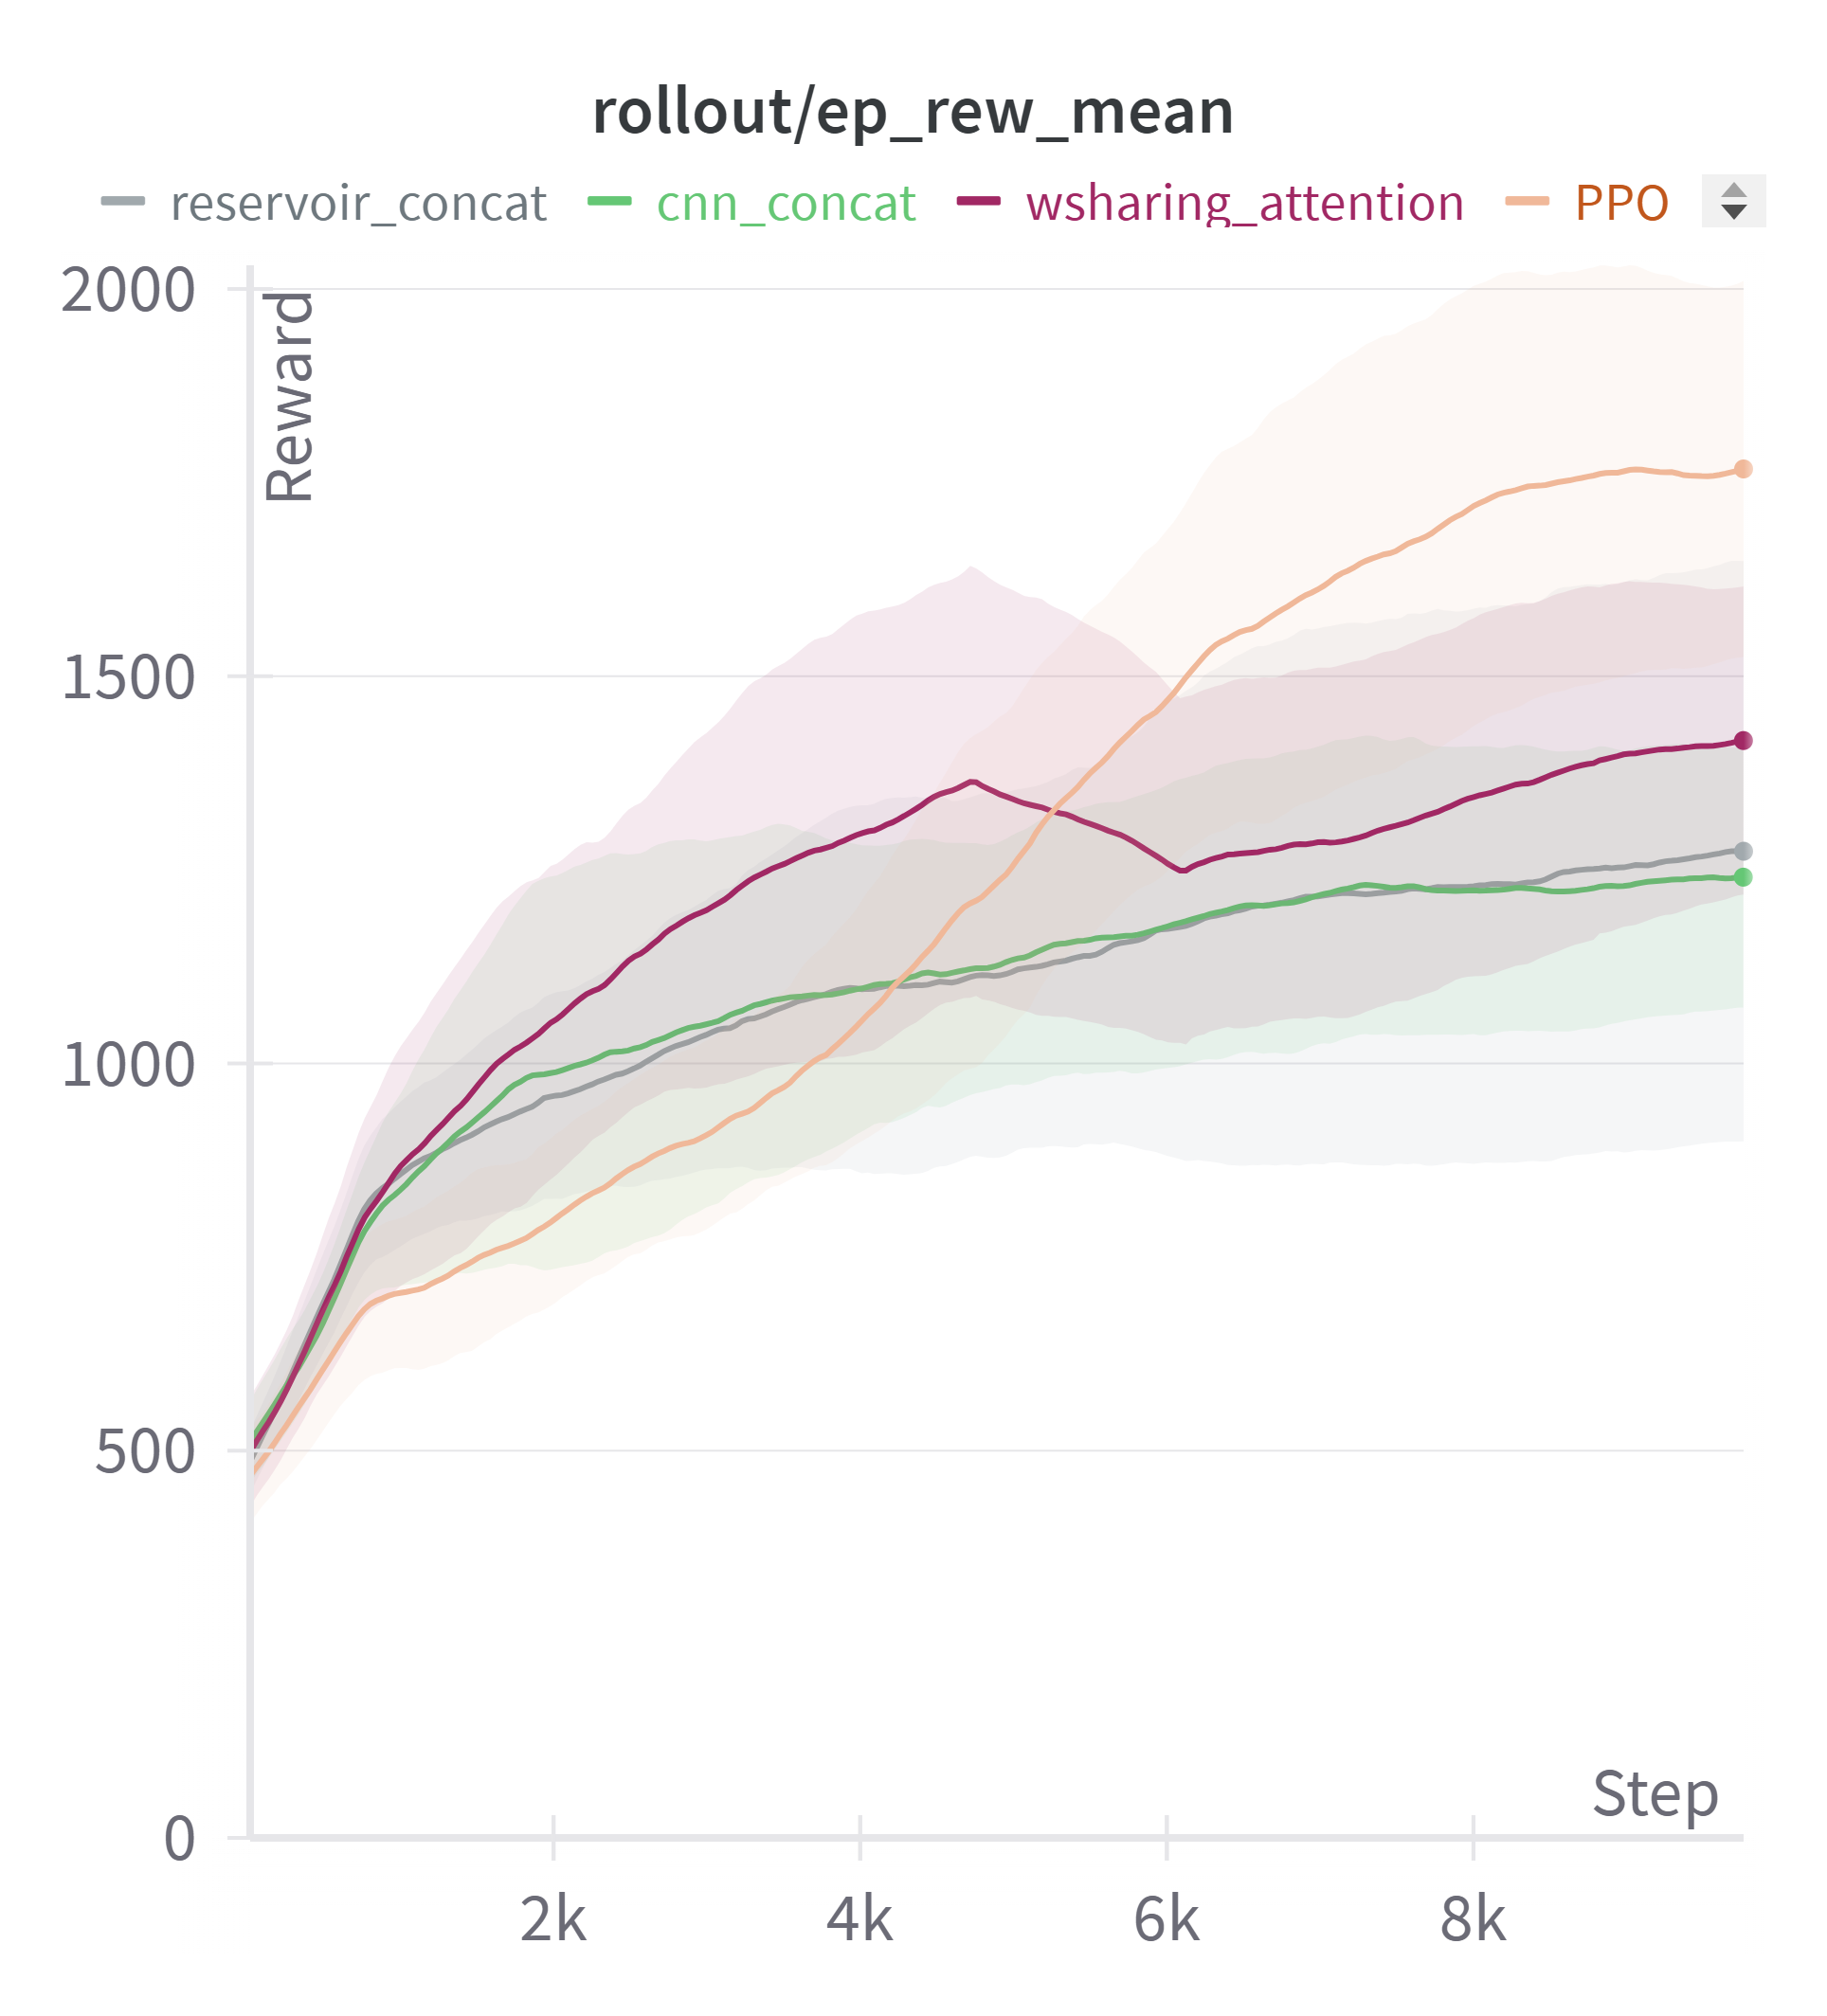
\includegraphics[width=\textwidth]{images/mspacman_train.png}
        \caption{\texttt{DPA}}
        \label{fig:dpa}
    \end{subfigure}

    \caption{n Figure we show the architecture of the Reservoir Combination Module (RES) and the DotProduct Attention Combination Module (DPA). In RES, we use reservoir dynamics to encode information coming from different FMs. In DPA, the embeddings are mapped into an embedding of fixed dimensions using $k$ different linear layers with the same size and we use State Encoder $\varepsilon$ as context \textit{C} as for WSA.}
    \label{fig:dpa_combination}
\end{figure}

